
\section{Simulation workflow}
\label{sec:simulation_workflow}


\subsection{Xsuite tracking data}
The first part of the data-generation workflow uses Xsuite-style tracking to produce paired input--output clouds. For each sample index $s$, one draws a parameter vector $\mu^{(s)}$ and an input beam family, samples a cloud
\begin{equation}
    Z_{\mathrm{in}}^{(s)}=\{\xi_i^{(s)}\}_{i=1}^{N_p},
\end{equation}
and tracks it through the lattice to obtain
\begin{equation}
    Z_{\mathrm{out}}^{(s)}=\Phi_{\mu^{(s)}}\big(Z_{\mathrm{in}}^{(s)}\big).
\end{equation}
The resulting dataset consists of tuples
\begin{equation}
    \mathcal{D}_{\mathrm{track}}=\left\{\big(Z_{\mathrm{in}}^{(s)},\mu^{(s)},Z_{\mathrm{out}}^{(s)}\big)\right\}_{s=1}^{N_s}.
    \label{eq:tracking_dataset_revised}
\end{equation}
In preliminary tests, $\mu$ may represent quadrupole strengths or other lattice-control parameters. In collective-effects studies, the natural parameters include bunch current, vacuum chamber radius, material resistivity, RF parameters, impedance scaling factors, and synchrotron tune.

\subsection{PyColleff-based longitudinal data}
For longitudinal collective-effects studies, synthetic data are generated by sampling machine and material parameters
\begin{equation}
    \mu^{(s)}=\big(I_b^{(s)},R^{(s)},\rho_{\mathrm{mat}}^{(s)},\ldots\big),
\end{equation}
then solving or approximating the self-consistent longitudinal response. The induced voltage may be written spectrally as
\begin{equation}
    V_{\mathrm{ind}}(z)=-\mathcal{F}^{-1}\left[Z_{\parallel}(\omega)\widehat{\lambda}(\omega)\right](z),
    \label{eq:induced_voltage_revised}
\end{equation}
and the total voltage is
\begin{equation}
    V_{\mathrm{tot}}(z)=V_{\mathrm{RF}}(z)+V_{\mathrm{ind}}[\lambda](z).
\end{equation}
A truncated fixed-point relaxation may then be written as
\begin{equation}
    \lambda^{(k+1)}=(1-\alpha)\lambda^{(k)}+\alpha\mathcal{T}_{\mu}\big(\lambda^{(k)}\big),
    \label{eq:pycolleff_relaxation_revised}
\end{equation}
where $\alpha\in(0,1)$ is an under-relaxation parameter. After $K$ iterations, the output profile is defined as $\lambda_{\mathrm{out}}=\lambda^{(K)}$. This produces paired data
\begin{equation}
    \mathcal{D}_{\lambda}=\left\{\big(\lambda_{\mathrm{in}}^{(s)},\mu^{(s)},\lambda_{\mathrm{out}}^{(s)}\big)\right\}_{s=1}^{N_s}.
\end{equation}

\subsection{Computational cost}
The motivation for surrogate modelling should be made explicit by documenting the computational cost of the reference pipeline. Table~\ref{tab:simulation_cost_template} is a template to be filled with measured values.

\begin{table}[H]
\centering
\caption{Template for reporting the computational cost of the simulation pipeline. Replace the dashes with measured values.}
\label{tab:simulation_cost_template}
\begin{tabular}{lcccc}
\toprule
Data source & Samples & Particles / grid & Time per sample & Total time \\
\midrule
Xsuite tracking & --- & --- & --- & --- \\
PyColleff longitudinal solver & --- & --- & --- & --- \\
6D histogram generation & --- & --- & --- & --- \\
\bottomrule
\end{tabular}
\end{table}

\subsection{Data representation}
\subsubsection{Empirical measures and reduced profiles}
A particle cloud defines an empirical measure
\begin{equation}
    \rho^N=\frac{1}{N_p}\sum_{i=1}^{N_p}\delta_{\xi_i}.
\end{equation}
For reduced longitudinal tasks, the cloud is projected onto a one-dimensional grid to form
\begin{equation}
    \lambda^h=\big(\lambda(\zeta_1),\ldots,\lambda(\zeta_{N_\zeta})\big)\in\mathbb{R}^{N_\zeta}.
\end{equation}
This is the natural input representation for the one-dimensional FNO baseline.

\subsubsection{Fifteen pairwise phase-space projections}
For the six-dimensional problem, directly representing the full density on a grid is infeasible. Instead, the beam is represented through the fifteen pairwise two-dimensional marginals associated with the coordinate pairs
\begin{equation}
    \mathcal{P}=\{(i,j):1\le i<j\le 6\}.
\end{equation}
The histogram representation is therefore
\begin{equation}
    \mathcal{H}(\rho)\in\mathbb{R}^{15\times N_b\times N_b},
    \label{eq:histogram_representation_revised}
\end{equation}
where $N_b$ is the number of bins per dimension. In addition, low-order physical descriptors are stored, including centroids and RMS sizes,
\begin{equation}
    m_i=\langle \xi_i\rangle,\qquad \sigma_i=\sqrt{\langle(\xi_i-m_i)^2\rangle}.
\end{equation}
This dual representation is important: the histograms preserve projected shape information, while the moments preserve global physical scale and extension. In the final implementation, these observables are used both for conditioning and for auxiliary prediction heads.

\begin{figure}[H]
    \centering
    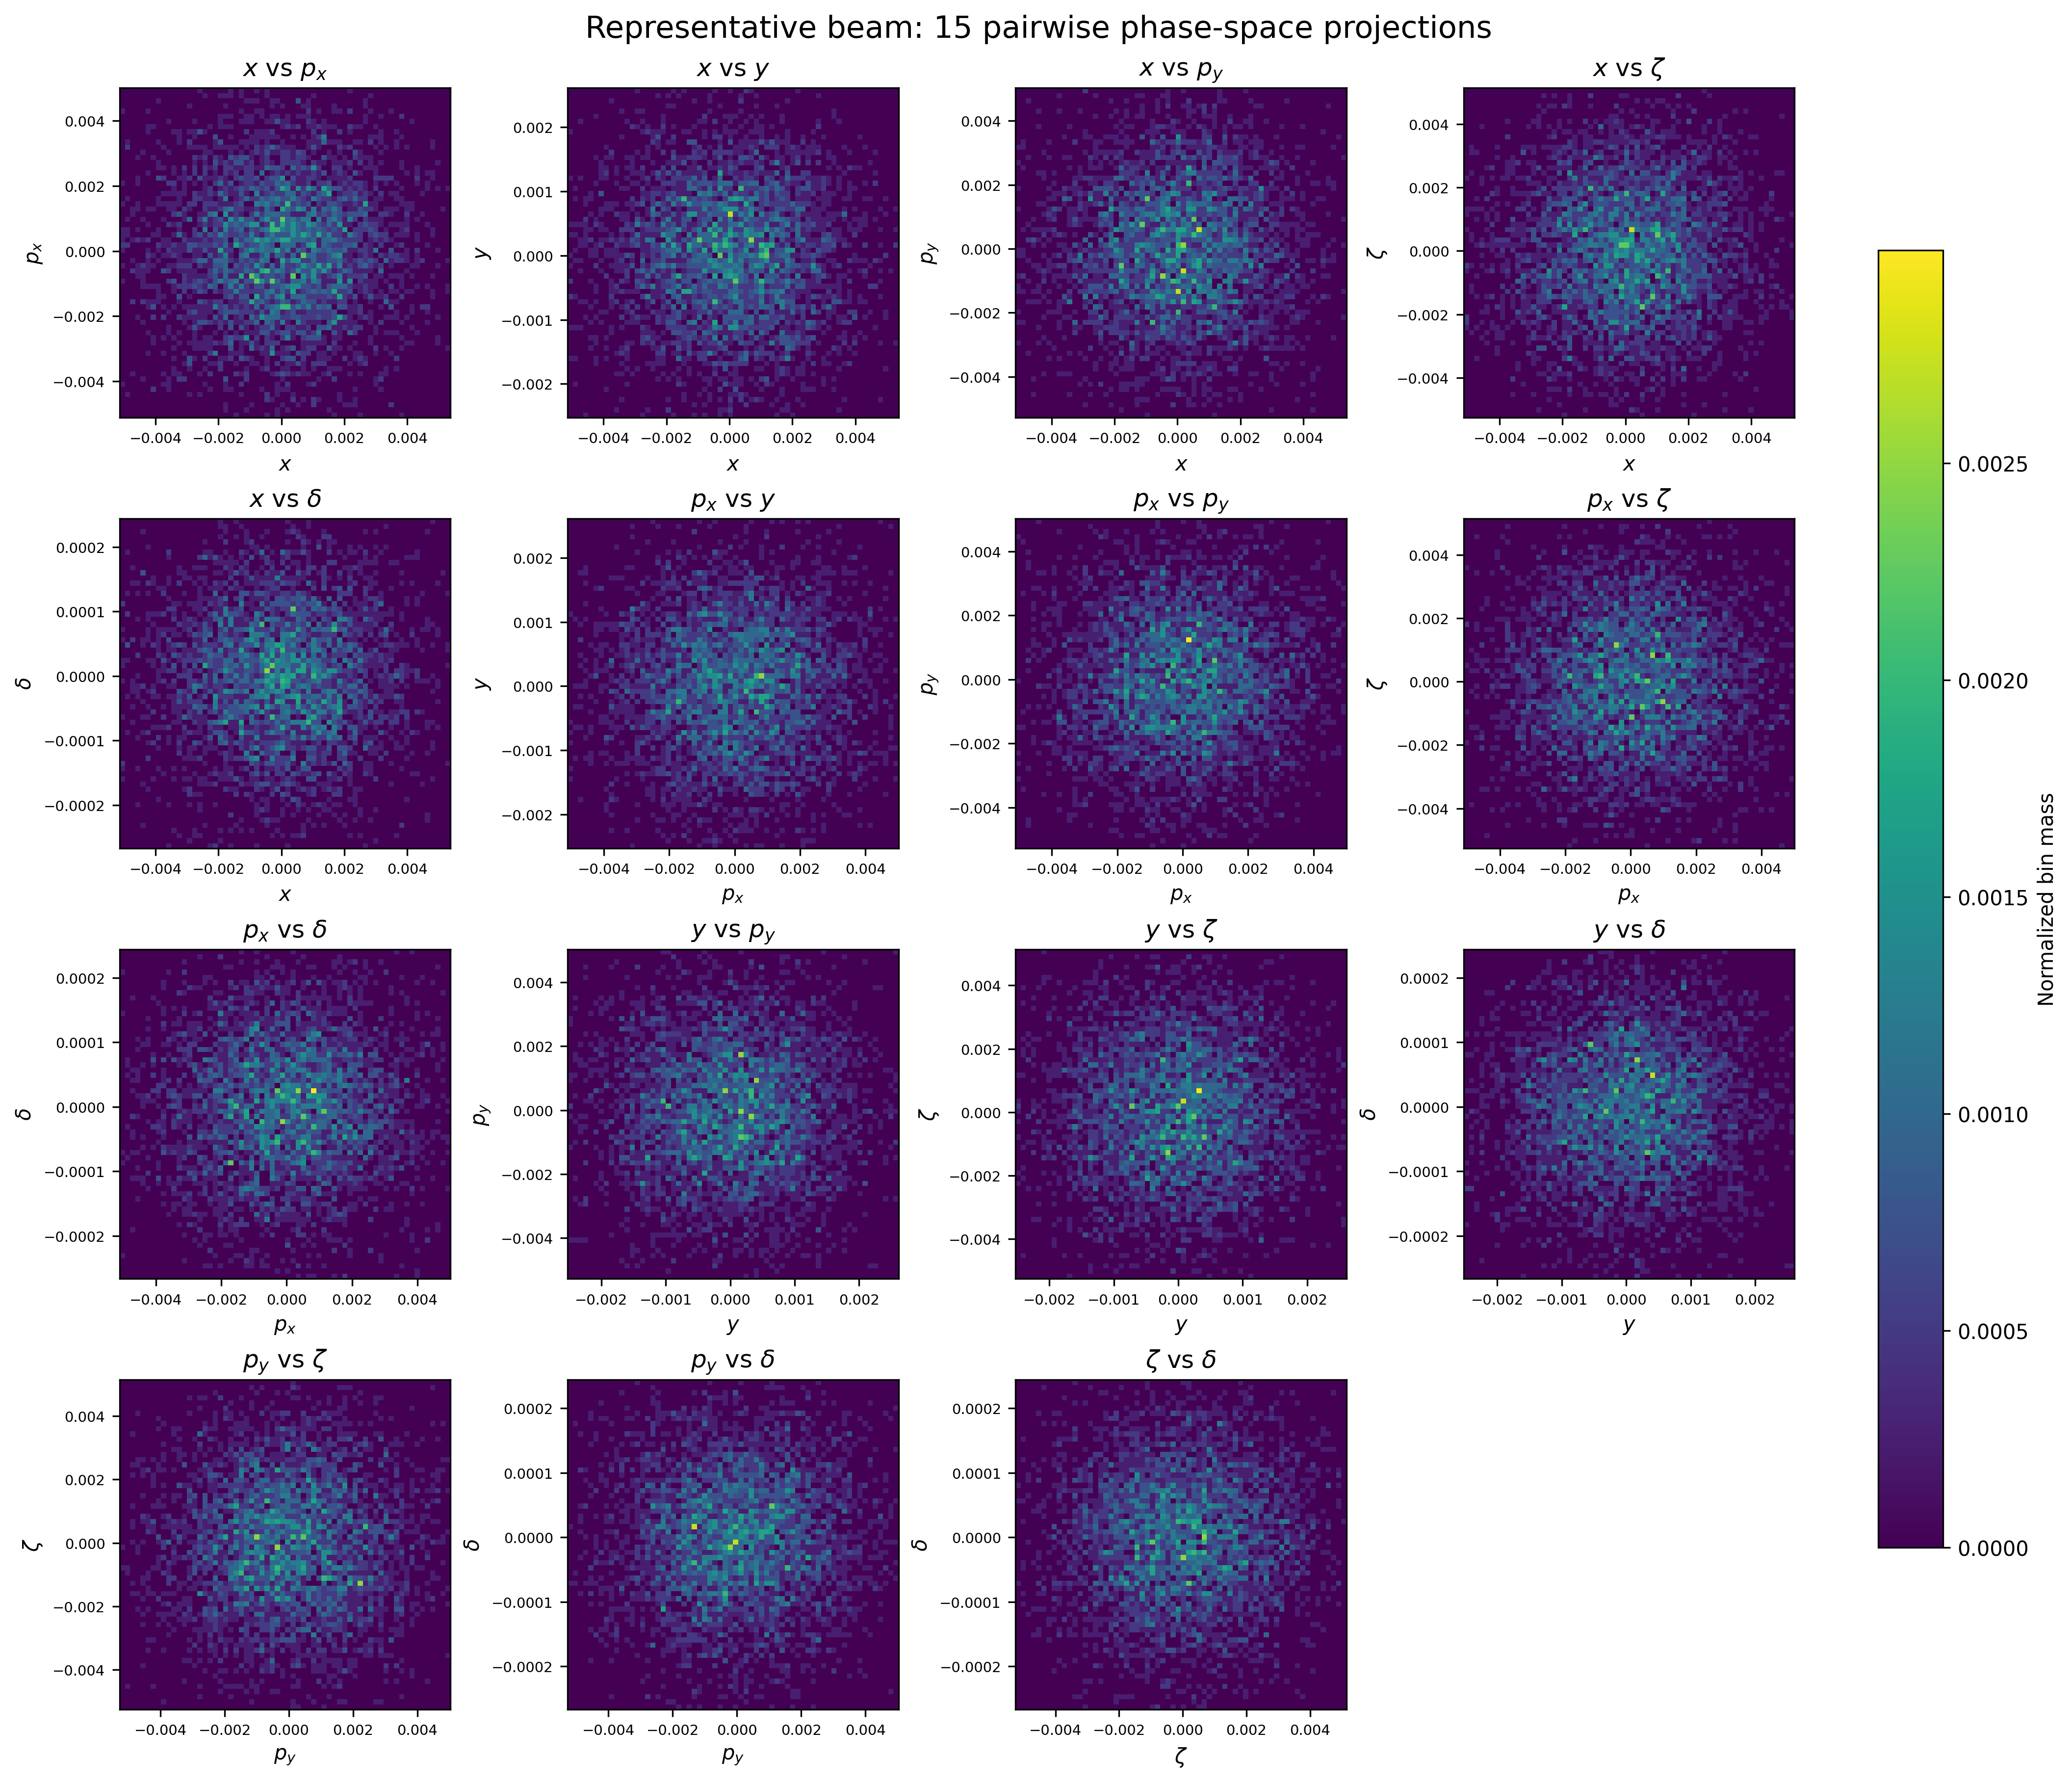
\includegraphics[
        width=\textwidth
    ]{images/generated/dataset_representation.png}
    \caption{
        Representative six-dimensional beam distribution encoded through its
        fifteen pairwise two-dimensional phase-space histograms. The associated
        centroid and RMS vectors provide complementary low-order physical
        descriptors of the beam position and spatial extension. This combined
        representation defines the distributional and physical information used
        by the CVAE-based surrogate model.
    }
    \label{fig:dataset_representation}
\end{figure}
% =============================================================================
